\documentclass[11pt]{article}
\usepackage[a4paper]{geometry}
\usepackage{mathtools,amssymb,amsthm}
\usepackage{polyglossia}
\usepackage{fontspec}
\usepackage{unicode-math}
\usepackage{titling}
\usepackage{tikz}
\usepackage[shortlabels]{enumitem}

\setdefaultlanguage{french}
\frenchspacing
\setmathfont{Latin Modern Math}
\setmathfont[range={\mathbb,\mathcal,\mathsf}]{xits-math.otf}

\let\oldepsilon\epsilon
\renewcommand\epsilon\varepsilon
\renewcommand\phi\varphi
\newcommand{\N}{\mathbb N}
\newcommand{\Z}{\mathbb Z}
\newcommand{\R}{\mathbb R}
\newcommand{\Q}{\mathbb Q}
\newcommand{\CC}{\mathbb C}
\newcommand{\K}{\mathbb K}

%% Theorem environments
\theoremstyle{definition}
\newtheorem{defn}{Définition}[section]
\newtheorem{prop}[defn]{Proposition}
\newtheorem{axio}[defn]{Axiome}
\newtheorem{exe}{Exemple}
\newtheorem{exo}{Exercice}

\theoremstyle{remark}
\newtheorem{rem}{Remarque}


\begin{document}

\begin{center}
	\hrulefill\\
    \vspace{6mm}
	\textsc{\LARGE Logique \& Ensembles}\\
    \vspace{3mm}
    \hrulefill
\end{center}
\vspace{1cm}

\begin{flushright}
\textit{<< La logique est l'hygiène des mathématiques. >>} \hfill— André Weil\end{flushright}

\begin{flushleft}
\textit{<<
	Plus il y a de fromage, plus il y a de trous.\\
	Plus il y a de trous, moins il y a de fromage.\\
	Donc plus il y a de fromage, moins il y a de fromage.
	 >>}\hfill — Paradoxe du Gruyère
\end{flushleft}

\begin{flushleft}
\textit{<< Tout ce qui est rare est super cher,\\
    Une Maserati à 20 euros, c'est rare,\\
    Donc une Maserati à 20 euros, c'est super cher >>.}\hfill — Bruce Benamran
\end{flushleft}

\begin{flushleft}
\textit{<< La mathématique est une science dangereuse : elle dévoile les supercheries et les erreurs de calculs. >>} \hfill — Galilée
\end{flushleft}

\vspace{1em}
Ce cours a pour objet de servir de fondement pour la compréhension de la logique formelle et du langage ensembliste et de leur utilisation en mathématiques au niveau lycée, permettant ainsi de poser les bases de la construction d'une démonstration mathématique.

%\tableofcontents

\section{Logique}

\subsection{Propositions, formules}

\begin{defn}[Proposition]
Une \textit{proposition} est la donnée d'une affirmation $P$. Elle peut prendre deux valeurs de vérité : le \textit{Vrai} ($V$) et le \textit{Faux} ($F$).
\end{defn}

\begin{exe}\leavevmode
\begin{enumerate}
\item << Aristote est mortel. >>
\item << Aristote est un chat. >>
\item << Les lois de la physique d'Aristote sont vraies. >>
\end{enumerate}
\end{exe}

\begin{defn}[Formule propositionnelle]
On peut partir des propositions de base dont on dispose pour construire des \textit{formules}, en les combinant avec des symboles appelés \textit{connecteurs logiques}.

C'est donc la donnée d'une expression où sont articulées des propositions à l'aide de connecteurs. Elles sont en soi des propositions.
\end{defn}

On verra plus loin quels sont ces symboles qui permettent d'articuler des propositions pour créer une formule.



La logique usuelle obéit au principe suivant (on peut décider de ne pas l'adopter, ce qui donne lieu à d'autres systèmes de logique bizarres étudiés par des chercheurs en logique...):

\begin{axio}[Principe du tiers exclu]
Une proposition prend la valeur \textit{Vrai} ou la valeur \textit{Faux}, \textbf{jamais les deux}.
\end{axio}

\begin{defn}[Identité de deux propositions]
Deux formules $P$ et $Q$ sont dites \textit{équivalentes} ou \textit{identiques} si elles ont toujours même valeur de vérité, quelles que soient les valeurs de vérité des variables qui y interviennent. On note
\[P\equiv Q
\]
\end{defn}

\begin{exe}\leavevmode
<< Aristote n'est pas mortel >> $\equiv$ << Aristote est immortel >>
\end{exe}

\begin{rem}Vous remarquerez qu'on ne se préoccupe pas de la véracité de ces propositions... Juste qu'elles reviennent à dire la même chose.
\end{rem}

\begin{defn}[Table de vérité]
La table de vérité d'une formule est un tableau dans lequel sont listées les valeurs de vérité de cette formule en fonction de celles des propositions qui y interviennent.
\end{defn}






\subsection{Opérateurs logiques}

\subsubsection{Négation}

\begin{defn}[Négation]
Soir $P$ une proposition. On appelle \textit{négation de $P$} et on note $\neg P$ la proposition de valeur de vérité opposée à $P$: quand $P$ est vraie, $\neg P$ est fausse, et vice-versa. Sa table de vérité est donnée par
\begin{center}
  \begin{tabular}{|c|c|}\hline
  $P$ & $\neg P$ \\ \hline
  $V$ & $F$ \\ \hline
  $F$ & $V$ \\ \hline
  \end{tabular}
\end{center}
\end{defn}

\begin{prop}
Soit $P$ une proposition. Alors
\[\neg\neg P \equiv P.
\]
\end{prop}

\begin{exe}\leavevmode\begin{enumerate}
\item $\neg$<< Aristote est mortel >> $\equiv$ << Aristote est immortel >>
\item $\neg$<< Aristote est un chat >> $\equiv$ << Aristote n'est pas un chat >>
\item $\neg$<< J'aime les frites >> $\equiv$ << \hspace{7cm} >>
\end{enumerate}

\end{exe}


\subsubsection{Conjonction}

\begin{defn}[Conjonction]
On appelle \textit{conjonction} et on note $\land$ l'opérateur dont la table est donnée par

\begin{table}[!ht]
\centering
\begin{tabular}{|c|c|c|}\hline
$P$ & $Q$ & $P\land Q$ \\ \hline
$V$ & $V$ & $V$ \\\hline
$V$ & $F$ & $F$ \\\hline
$F$ & $V$ & $F$ \\\hline
$F$ & $F$ & $F$ \\\hline
\end{tabular}
\end{table}

$P\land Q$ se lit << $P$ et $Q$ >>.
\end{defn}

\begin{exe}
<< Aristote est mortel >> $\land$ << Aristote est un chat >> est ...\\
<< Tous les hommes sont mortels >> $\land$ << Tous les hommes sont mortels >> $\equiv$ ...\\
<< Ce mammifère est un chat >>$\land $ << Ce mammifère n'est pas un chat >> est...
\end{exe}

\begin{rem} Observez que dans le dernier cas, on peut conclure sans rien vraiment savoir sur le mammifère en question !
\end{rem}

\begin{prop}
Soient $P,Q,R$ des propositions.
\begin{enumerate}
\item $(P\land Q)\land R \equiv P\land (Q\land R)$
\item $P\land Q \equiv Q\land P$
\item $P\land P\equiv P$
\item $P\land \neg P \equiv F$ (principe du tiers exclu)
\end{enumerate}

\end{prop}



\subsubsection{Disjonction}

\begin{defn}[Disjonction]
On appelle \textit{disjonction} et on note $\lor$ l'opérateur dont la table est donnée par
\begin{table}[ht]
\centering
\begin{tabular}{|c|c|c|}\hline
$P$ & $Q$ & $P\lor Q$ \\ \hline
$V$ & $V$ & $V$ \\\hline
$V$ & $F$ & $V$ \\\hline
$F$ & $V$ & $V$ \\\hline
$F$ & $F$ & $F$ \\\hline
\end{tabular}
\end{table}

$P\lor Q$ se lit << $P$ ou $Q$ >>.
\end{defn}

\begin{prop}
Soient $P,Q,R$ des propositions.
\begin{enumerate}
\item $(P\lor Q)\lor R \equiv P\lor (Q\lor R)$
\item $P\lor Q \equiv Q\lor P$
\item $P\lor P\equiv P$
\item $P\lor \neg P\equiv V$ (principe du tiers exclu, encore)
\end{enumerate}
\end{prop}



\subsubsection{Implication, équivalence}

\begin{defn}[Implication]
L'opérateur \textit{implication}, noté $\Rightarrow$, a pour table de vérité

\begin{table}[ht]
\centering
\begin{tabular}{|c|c|c|}\hline
$P$ & $Q$ & $P\Rightarrow Q$ \\ \hline
$V$ & $V$ & $V$ \\\hline
$V$ & $F$ & $F$ \\\hline
$F$ & $V$ & $V$ \\\hline
$F$ & $F$ & $V$ \\\hline
\end{tabular}
\end{table}

$P\Rightarrow Q$ se lit << $P$ implique $Q$ >>.
\end{defn}

\begin{exe}
	Tous les hommes sont mortels.\\
	Or Socrate est un homme.\\
	Donc Socrate est mortel.
\end{exe}

\begin{defn}[Équivalence]
L'opérateur \textit{équivalence}, noté $\Leftrightarrow$, a pour table de vérité

\begin{table}[ht]
\centering
\begin{tabular}{|c|c|c|}\hline
$P$ & $Q$ & $P\Leftrightarrow Q$ \\ \hline
$V$ & $V$ & $V$ \\\hline
$V$ & $F$ & $F$ \\\hline
$F$ & $V$ & $F$ \\\hline
$F$ & $F$ & $V$ \\\hline
\end{tabular}
\end{table}

$P\Leftrightarrow Q$ se lit << $P$ équivaut à $Q$ >>
\end{defn}




\subsubsection{Quelques équivalences de formules}

\begin{prop}[Distributivités]\leavevmode
\begin{enumerate}
\item $P\land (Q\lor R) \equiv(P\land Q)\lor (P\land R)$
\item $P\lor(Q\land R)\equiv (P\lor Q)\land (P\lor R)$
\end{enumerate}

\end{prop}

\begin{prop}[Négation d'une formule, lois de De Morgan]\leavevmode
\begin{enumerate}
\item $\neg(P\land Q) \equiv (\neg P)\lor(\neg Q)$ (loi de De Morgan)
\item $\neg(P\lor Q) \equiv (\neg P)\land (\neg Q)$ (deuxième loi de De Morgan)
\item $\neg(P\Rightarrow Q)\equiv P\land\neg Q$.
\item $\neg(P\Longleftrightarrow Q) \equiv P\Longleftrightarrow (\neg Q) \equiv (\neg P) \Longleftrightarrow Q$
\end{enumerate}
\end{prop}

\begin{rem}
Le point 3. donne un moyen simple de contredire une implication.
\end{rem}

\begin{exe}
On peut montrer que l'affirmation << si le sol est mouillé alors il pleut >> est fausse. En effet, elle se réécrit << le sol est mouillé >> $\Rightarrow $ << il pleut >>, et comme on peut avoir << le sol est mouillé >> et << il ne pleut pas >> (il suffit d'arroser le sol quand il fait beau...), on a un contre-exemple.
\end{exe}

\begin{prop}\leavevmode
\begin{enumerate}
\item $P\Longrightarrow Q\equiv (P\Longrightarrow Q)\land(Q\Longrightarrow P)$ (principe de double implication)
\item $(P\Rightarrow Q)\equiv (\neg Q\Rightarrow \neg P)$ (principe de la contraposée)
\item $(P\lor Q)\Rightarrow R\equiv (P\Rightarrow R)\land (Q\Rightarrow R)$ (disjonction de cas)
\item $P\Rightarrow Q \equiv \neg P\lor Q$
\item $(P\land (P\Rightarrow Q))\Rightarrow Q\equiv V$ (\textit{modus ponens} 
\item $P\Rightarrow(Q\lor R) \equiv (P\land \neg Q)\Rightarrow R $
\end{enumerate}
\end{prop}

\begin{exo}[D]
Niez:\begin{enumerate}
\item $((A\Rightarrow B)\land C)\lor\neg B$
\item $(((A\Leftrightarrow B)\lor C)\Rightarrow B)\Leftrightarrow A$
\end{enumerate}
\end{exo}

\subsection{Formules quantifiées}

Maintenant, on va apprendre à manier des variables dans des formules logiques.

\begin{defn}[Prédicat]
On appelle \textit{prédicat} une articulation de relations faisant intervenir des variables.
\end{defn}

\begin{defn}[Quantificateur universel]
Le quantificateur universel $\forall$, lu << pour tout >> ou << quel que soit >>, est défini comme suit: la proposition
\[ \forall x,P(x)\]
est vrai si $P(x)$ est vrai quelle que soit la valeur prise par $x$.
\end{defn}

\begin{prop}
	$\neg(\forall x,P(x)) \equiv \exists x,\neg P(x)$
\end{prop}

\begin{exe}
	$\neg$(<< Tous les bretons sont des indépendantistes >>) $\equiv$ << Il existe un breton qui n'est pas indépendantiste >>.
\end{exe}

\begin{defn}[Quantificateur existentiel]
Le quantificateur existentiel $\exists$, lu << il existe >>, est défini comme suit: le prédicat
\[ \exists x,P(x)\]
est vrai si la proposition $P(x)$ est vraie pour un certain $x$. Dans ce cas, on peut se donner un $x$ qui vérifie $P(x)$, même si on ne peut pas l'expliciter...
\end{defn}

\begin{rem}
	Quand une variable est quantifiée dans une expression, on dit qu'elle est \textit{liée} ou \textit{muette}. Sinon, elle est \textit{libre}. Par exemple, dans
	\[ \forall x,x+y \geq 0, \]
	$x$ est liée et $y$ est libre.
	
	On peut changer le nom d'une variable muette. En l'occurrence, on peut changer $x$ par $z$ dans ce qui précède:
	\[ \forall x,x+y \geq 0 \]
	est la même chose que
	\[ \forall z,z+y \geq 0. \]
\end{rem}

\begin{prop}
	$\neg(\exists x,P(x))\equiv \forall x,\neg P(x). $
\end{prop}

\begin{exe}\begin{enumerate}
		\item $P(x) :$ << $x \geq 2 \Rightarrow x^2 \geq 4$ >> est un prédicat, faisant intervenir les relations << $x^2\leq 0$ >> et << $ x=0$ >>.
		
		On a que la proposition $\forall x,P(x)$ est vraie. Elle s'écrit $\forall x,\ x\geq 2\Rightarrow x^2\geq 4 $, ce qui se réécrit, par abus de notation,
		\[ \forall x\geq2,\ x^2\geq 4. \]
		
		En général, une proposition de la forme $\forall x,\ x\in E\Rightarrow Q(x)$, peut se réécrire
		\[ \forall x\in E,\ Q(x). \]
		
		\item La proposition $\exists x,\ x\geq 0\land x^2=4 $, où intervient le prédicat $P(x):$ << $x\geq 0\land x^2=4 $ >>, se réécrit
		\[ \exists x\geq 0,\ x^2=4. \]
	\end{enumerate}	
\end{exe}

\begin{prop}\leavevmode
	\begin{enumerate}
		\item $\forall x,(P(x)\land Q(x))\equiv (\forall x,P(x))\land (\forall x,Q(x)) $.
		\item $\exists x,(P(x)\lor Q(x))\equiv (\exists x,P(x))\lor(\exists x,Q(x)). $
	\end{enumerate}
\end{prop}


%%%%%%%%%%%%%%%%%%%%

\section{Comment écrire une démonstration}

Donnons quelques méthodes pour rédiger proprement une démonstration mathématique dans les règles de l'art — c'est-à-dire de façon correcte du point de vue logique, et structurée.

D'abord, il faut décomposer l'énoncé que l'on veut montrer en des propositions plus simples. D'habitude, l'énoncé s'écrit $H\Rightarrow C$
où $H$ contient les hypothèses, $C$ les conclusions. Il faut donc déconstruire $H$ et $C$ en des blocs que l'on peut traiter séparément, et recoller pour montrer ce que l'on veut.

\begin{prop}[Montrer $A\land B$]
	Montrer séparément qu'on a $A$, et qu'on a $B$.
\end{prop}

\begin{prop}[Montrer une implication $A\Rightarrow B$]
	
	
	D'abord supposer $A$, ce que l'on peut écrire << supposons $A$ vraie >>, et ensuite montrer qu'on a $B$ en utilisant les règles...

	Cela s'appelle montrer l'implication directe. On peut aussi ruser, et démontrer que $\neg B\Rightarrow \neg A$, puisque c'est la même chose que $A\Rightarrow B$.
\end{prop}

\begin{prop}[Montrer une équivalence $A\Leftrightarrow B$]
	
	
	Typiquement, on peut montrer que $A\Rightarrow B$ (ce que l'on appelle le \textit{sens direct}), puis que $B\Rightarrow A$ (ce que l'on appelle le \textit{sens réciproque}).
	
	On peut aussi essayer d'enchaîner des équivalences assez évidentes, en justifiant éventuellement les moins évidentes par une précision entre parenthèses, un << puisque >>, ou encore un participe présent du style << $x\longmapsto x^2$ étant croissante sur $\R^+$ >>... Mais il faut faire attention à ce que cela ne nuise pas à la clarté de la démonstration.
\end{prop}

\begin{prop}[Montrer que $\forall x, A(x)$]
	Il faut montrer que quel que soit $x$, $A(x)$ est vraie. Pour cela, on pose un $x$ quelconque, on suppose qu'il vérifie les hypothèses de $A(x)$ et en on montre la conclusion.
\end{prop}

\begin{prop}[Montrer $A\lor B$]
	Il faut montrer que l'on a soit $A$, soit $B$... donc que si on n'a pas $A$, alors on aura nécessairement $B$. Il suffit donc de montrer l'implication $\neg A\Rightarrow B$.
\end{prop}

\begin{prop}[Montrer $\exists x,A(x)$]
	On peut s'y prendre de plusieurs façons. On peut essayer d'exhiber un $x$ qui vérifie $A(x)$. Par exemple, pour montrer qu'il existe $x$ tel que $x^2=4$, on peut prendre $x=2$ et on a fini. 
	
	Si on n'y parvient pas, on peut essayer de le construire à la main. C'est loin d'être toujours facile.
	
	On peut des fois conclure en utilisant des théorème du cours donnant l'existence directement.
\end{prop}

\begin{exo}[M]
	Montrer que si $n$ est un entier, $n$ est pair si et seulement si $n^2$ est pair.
\end{exo}

\begin{proof}
	On décompose l'énoncé de la façon suivante:
	\[ \forall n,n\text{ entier}\Rightarrow (n\text{ pair}\Leftrightarrow n^2\text{ pair}) \]
	ou encore, avec l'abus de notation usuel:
	\[ \forall n\text{ entier},(n\text{ pair}\Leftrightarrow n^2\text{ pair}). \]
	
	Pour démontrer l'implication, il faut se donner son hypothèse: soit $n$ un entier. Ensuite, il faut démontrer le deuxième bloc, le résultat << $n$ pair $\Leftrightarrow$ $n^2$ pair >>.
	
	Il s'agit d'une équivalence, donc on va procéder par double implication.
	
	\textbf{Le sens direct.} On va montrer l'implication << $n$ pair $\Rightarrow$ $n^2$ pair >>. On va utiliser la première méthode proposée. On suppose donc que $n$ est pair : il existe un entier $k$ tel que $n=2k$ (c'est la définition d'être pair). Alors $n^2=(2k)^2=2^2k^2=4k^2=2\times (2k^2)$, ce qui est pair.
	
	\textbf{Le sens réciproque.} On va montrer l'autre sens: << $n^2$ pair $\Rightarrow$ $n$ pair >>. Cela semble un peu corsé, donc on va plutôt montrer la contraposée: << $\neg(n\text{ pair})\Rightarrow \neg(n^2\text{ pair})$ >>.
	
	La négation de << être pair >> étant << être impair >>, cela revient à montrer que << $n$ impair $\Rightarrow$ $n^2$ impair >>. Cette implication paraît plus simple à montrer, donc on peut tenter de le faire directement: supposons $n$ impair. Alors il existe un entier $k$ tel que $n=2k+1$, et alors $n^2=(2k+1)^2=4k^2+4k + 1 = 2(2k^2+2k)+1$, ce qui est impair. D'où l'implication.
	
	Par contraposée on a bien << $n^2$ pair $\Rightarrow$ $n$ pair >>.
\end{proof}


\section{Ensembles}

\subsection{Généralités}

\begin{defn}
	Un ensemble $E$ est une \textit{collection} d'objets $x$, que l'on appelle \textit{éléments de $E$}. Si $x$ est un élément de $E$, on dit que << $x$ appartient à $E$ >> et on note \[x\in E.\]
Si au contraire $x$ n'appartient pas à $E$, on notera
    \[x\not\in E.\]
\end{defn}

\begin{rem}
La notation $\in$ est introduite en 1890 par le mathématicien italien \textsc{Péano}. C'est en fait une variante de la lettre grecque $\oldepsilon$ << epsilon >> (cinquième lettre, donc le << e >>, de l'alphabet grec), pour \textit{esti}, << est >> en italien.
\end{rem}

\begin{rem} Cette notion est insuffisante à cause du paradoxe de \textsc{Russel}. Il peut s'énoncer ainsi : on appelle barbier toute personne se rasant les personnes qui ne se rasent pas elles-mêmes. Alors, le barbier se rase-t-il lui même ? Si c'est le cas, alors le barbier rase une personne qui se rase elle-même. Sinon, le barbier fait partie de ces personnes qui ne se rasent pas par elles-mêmes, donc qui devraient être rasées par le barbier...
\end{rem}

Bien sûr, on peut argumenter avec la plausibilité d'une telle situation, construite de toute part pour qu'il y ait un problème... La version formelle du paradoxe de Russel, par contre, est indiscutable:

\theoremstyle{plain}
\newtheorem*{paradox}{Paradoxe}
\begin{paradox}[de \textsc{Russel}]
Soit $R$ l'ensemble de tous les ensembles $X$ qui n'appartiennent pas à eux mêmes. On peut le définir, puisqu'un ensemble est une collection d'objets... Ainsi, un ensemble $X$ appartient à $R$ si et seulement si $X\not\in X$.

Alors, on est en droit de se poser la question: est-ce que $R\in R$ ?
\end{paradox}

Pour se sortir de ce bourbier, on impose de plus la condition suivante:
\[\textbf{Un ensemble ne peut se contenir lui-même.}\]

\begin{defn}[Ensemble vide]
L'ensemble vide, noté $\emptyset$, est l'ensemble ne contenant aucun élément.
\end{defn}

\begin{defn}
On dit que deux ensembles $E$ et $F$ sont \textit{égaux} si tous les éléments de l'un appartient à l'autre et réciproquement:
\[
x\in E\Longleftrightarrow x\in F.
\]
On note classiquement
\[ E = F. \]
\end{defn}

\begin{defn}[Comment définir un ensemble]\leavevmode
\begin{itemize}
\item \textbf{Énumération} on donne tous les éléments de l'ensemble. Par exemple, on écrit
\[
E=\{x_1,x_2,\ldots,x_n\}
\]
Et il n'y a pas d'ordre d'énumération précis. De plus, un élément ne peut pas apparaître plusieurs fois.
\item \textbf{Compréhension} on donne un prédicat $P(x)$ qui caractérise les éléments de l'ensemble $E$: un élément $x$ appartient à $E$ si et seulment si $P(x)$ est vrai. On écrit alors:
\[ E = \{x\ |\ P(x)\} \]
où la barre verticale << | >> signifie << tel que >>. On peut aussi écrire << tel que >> en toutes lettres: $E = \{x\ \text{tel que}\ P(x)\}$.
\item \textbf{Induction structurelle} On \textit{induit} l'ensemble en donnant quelques éléments de base, des << briques >>, en quelque sorte, et des règles de construction pour former le reste des éléments. Comme construire un bâtiment!
\end{itemize}
\end{defn}

\begin{exe}\leavevmode
\begin{itemize}
\item \textbf{Énumération} $E=\{0,3,28,4,-10\}$
On aurait très bien pu écrire:
\[ \{-10,28,0,3,4\} \]
ou
\[ \{28,0,-10,4,3\} \]
ou
\[ \{28,4,28,0,0,0,0,4,-10,-10,3\} \]
et cela n'a n'aurait rien changé au sens. 

\item \textbf{Compréhension} $E = \{x\in\R\ |\ \exists y\in\R\quad x^2=y \}$. Quel est cet ensemble ?

Encore un autre exemple: $\{x\in\R\ |\ x^2-4x+1 \geq 0\}$.
\item \textbf{Induction structurelle} Surtout intéressant en algèbre et en informatique. On retiendra l'exemple des \textit{arbres binaires}. On se donne un élément d'origine, qui s'appelle \textit{racine} de l'arbre. Tout élément de l'arbre s'appelle un \textit{noeud}. Chaque noeud $x$ a au plus deux \textit{fils}, qui sont des noeuds associés. Réciproquement, si $y$ est un fils de $x$, $x$ est appelé le \textit{père} de $y$.
\begin{figure}
\centering
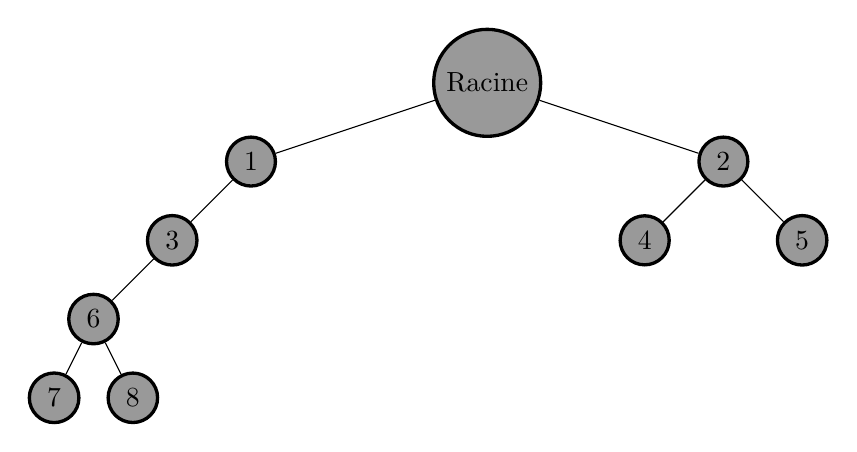
\begin{tikzpicture}[roundnode/.style={circle, draw=black!100, fill=black!40, very thick, minimum size=1mm}]
\node[roundnode] (Racine) at (0,0) {Racine};
\node[roundnode] (Fg) at (-3,-1) {1};
\node[roundnode] (Fd) at (3,-1) {2};
\node[roundnode] (Fdd) at (4,-2) {5};
\node[roundnode] (Fdg) at (2,-2) {4};
\node[roundnode] (Fgg) at (-4,-2) {3};
\node[roundnode] (Fggg) at (-5,-3) {6};
\node[roundnode] (Fgggg) at (-5.5,-4) {7};
\node[roundnode] (Fgggd) at (-4.5,-4) {8};
\draw (Racine) -- (Fg);
\draw (Racine) -- (Fd);
\draw (Fd) -- (Fdd);
\draw (Fd) -- (Fdg);
\draw (Fg) -- (Fgg);
\draw (Fgg) -- (Fggg);
\draw (Fggg) -- (Fgggg);
\draw (Fggg) -- (Fgggd);
\end{tikzpicture}
\caption{Ceci est un arbre. Les fils sont numérotés de gauche à droite avec priorité sur la profondeur.}
\end{figure}
\end{itemize}
\end{exe}

\subsection{Sous-ensembles}

\subsubsection{Définition}

\begin{defn}[Sous-ensemble]
Soit $E$ un ensemble, un \textit{sous-ensemble} de $E$ est un ensemble $F$ dont tous les éléments sont aussi des éléments de $E$:
\[ 
\forall x\quad x\in F\Longrightarrow x\in E.
\]
On dit que \textit{$F$ est inclus dans $E$} et on note
\[ F\subset E. \]
\end{defn}

\begin{prop}[Principe de double inclusion]
On a
\[E=F\]
si et seulement si
\[E\subset F\ \text{et}\ F\subset E.\]
\end{prop}

\begin{proof}
Provient du principe de double implication. En effet, quel que soit $x$, 
\[x\in E\Longleftrightarrow x\in F \quad\text{est exactement} \quad (x\in E\Longrightarrow x\in F)\ \text{et}\ (x\in F\Longrightarrow x\in E)\]
par principe de double implication. Ainsi, les conditions d'égalité de $E$ et $F$ et de double inclusion sont identiques. D'où l'équivalence.
\end{proof}

\begin{prop}
Soit $E$ un ensemble. Alors, l'ensemble vide $\emptyset$ est un sous-ensemble de $E$. C'est même le seul sous-ensemble de l'ensemble vide...
\end{prop}

\begin{prop}
Quel que soit $x$, l'implication
\[ x\in\emptyset \Rightarrow x\in E \]
est vraie, puisque $x\in\emptyset$ est toujours faux, et que Faux implique Vrai...
\end{prop}

\begin{defn}
On appelle \textit{singleton} un ensemble constitué d'un seul élément, c'est-à-dire de la forme
\[
\{x \}.
\]
\end{defn}

\begin{prop}
Soit $E$ un ensemble. On a $x\in E$ si et seulement si le singleton $\{x\}\subset E$.
\end{prop}

\subsubsection{Parties}

\begin{defn}
On appelle \textit{partie} d'un ensemble $E$ tout sous-ensemble $F$ de $E$. C'est une autre terminologie pour parler de sous-ensemble.

L'\textit{ensemble des parties de $E$} est noté $\mathcal P(E)$. On a alors l'équivalence suivante:
\[ F\in\mathcal P(E) \Longleftrightarrow F\subset E.\]
\end{defn}

On a notamment $E\in\mathcal P(E)$ et $\emptyset\in\mathcal P(E)$.

\subsection{Opérations sur les ensembles}

\subsubsection{Intersection}

\begin{defn}[Intersection]
Soient $E$ et $F$ deux ensembles. L'\textit{intersection} de $E$ et de $F$, notée
\[E\cap F\]
est l'ensemble des éléments appartenant à $E$ et à $F$ :
\[E\cap F = \{x\ |\ x\in E\land x\in F\}.\]
\end{defn}

On a les propriétés suivantes:

\begin{prop}
Soient $E$, $F$, $G$ trois ensembles. Alors:
\begin{enumerate}
\item $E\cap F=  F\cap E$
\item $(E\cap F)\cap G = E\cap (F\cap G)$
\item $E\cap F\subset E$ et $E\cap F\subset F$ et si $G$ vérifie aussi cette propriété, alors $G\subset E\cap F$ (propriété de maximalité).
\item $E\cap\emptyset= \emptyset$ d'après ce qui précède directement, ou en regardant les $x\in E\cap\emptyset$.
\item $F\subset E$, alors $E\cap F=F$.
\end{enumerate}
\end{prop}

Ces résultats proviennent directement des résultats de logique sur l'opérateur << et >> ($\land$).

\begin{defn}
Deux ensembles $E$ et $F$ sont dit disjoints si ils n'ont aucun élément en commun:
\[E\cap F =\emptyset. \]
\end{defn}

\subsubsection{Union}

\begin{defn}[Union]
Soient $E$ et $F$ deux ensembles. Leur \textit{union}, notée
\[E\cup F,\]
est l'ensemble de tous les éléments de $E$ ou de $F$ :
\[E\cup F = \{x\ |\ x\in E\lor x\in F\}. \]
\end{defn}

\begin{exe}\leavevmode
\begin{itemize}
\item $\R_{-} \cup \R_{+} = \R$
\end{itemize}
\end{exe}

on a les propriétés suivantes:

\begin{prop}
Soient $E$, $F$, $G$ trois ensembles.
\begin{itemize}
\item $E\cup F=F\cup E$.
\item $(E\cup F)\cup G = E\cup(F\cup G)$.
\item $E\subset E\cup F $ et $F\subset E\cup F$, et si $G$ vérifie aussi cette propriété, alors $E\cup F\subset G$ (propriété de minimalité).
\item $E\cup\emptyset = E$ d'après ce qui précède, ou en regardant les éléments.
\item Si $F\subset E$, alors $E\cup F= E$.
\end{itemize}
\end{prop}

Encore une fois, elles découlent des résultats de logique, cette fois-ci sur l'opérateur de disjonction << ou >> ($\lor$).

Le cours de logique amène également ces résultats, découlant des lois de De Morgan (distributivités entre le << et >> et le << ou >>).

\begin{prop}[Distributivités, loi de De Morgan]
Soient $E$, $F$ et $G$ trois ensembles. Alors:
\begin{itemize}
\item $E\cup(F\cap G) = (E\cup F)\cap(E\cup G)$.
\item $E\cap(F\cup G) = (E\cap F)\cup(E\cap G)$.
\end{itemize}
\end{prop}

\subsubsection{Complémentaire d'un ensemble dans un autre}

\begin{defn}[Complémentaire d'un ensemble]
Soit $E$ un ensemble, et $F$ un sous-ensemble de $E$. Le \textit{complémentaire} de $F$ dans $E$, noté
\[\complement_E F, \]
est l'ensemble des éléments de $E$ qui manquent à $F$, soit
\[\complement_E F = \{x\in E\ |\ x\not\in F\}. \]
\end{defn}

On a donc les deux propriétés assez évidentes, qui caractérisent en fait le complémentaire (c'est le seul à les vérifier):

\begin{prop}
Soit $E$ un ensemble et $F$ un sous-ensemble. Alors:
\begin{itemize}
\item $F$ et son complémentaire sont disjoints:
\[F\cap \complement_E F = \emptyset. \]
\item L'union de $F$ et son complémentaire fait $E$ tout entier:
\[ F\cup\complement_E F = E. \]
\end{itemize}
\end{prop}

\begin{defn}[Différence ensembliste]
Soient $E$ et $F$ deux ensembles quelconques. Alors, la différence de $E$ et $F$, notée
\[ E\backslash F, \]
est le complémentaire de $E\cap F$ dans $E$. C'est l'ensemble des éléments de $E$ qui ne sont pas aussi des éléments de $F$. Dans le cas où $F$ est un sous-ensemble de $E$, on retombe bien sur le complémentaire défini plus haut.
\end{defn}

\subsection{Cardinalité}

La question se pose tout de suite: étant donné un ensemble, combien d'éléments a-t-il ? Intuitivement, si l'ensemble est fini, dans le sens où on peut énumérer tous ses éléments (en temps fini), il suffit de les compter. Et si il est infini ?

\begin{defn}[Cardinal, notion intuitive]
Le \textit{cardinal} d'un ensemble $E$, noté $\mathrm{Card}(E)$ ou $|E|$, et la << taille >> de l'ensemble. Si l'ensemble est fini dans le sens donné ci-dessus, il s'agit du nombre d'éléments qui lui appartiennent.
\end{defn}

\begin{exe}\leavevmode
\begin{itemize}
\item $\mathrm{Card}(\emptyset) = 0$
\item $\mathrm{Card}(\{1\}) = 1$, $\mathrm{Card}(\emptyset\}) = 1$, et généralement le cardinal d'un singleton vaut $1$.
\item $\mathrm{Card}(\{ 1,3,-1,36\}) = \ldots$
\item $\mathrm{Card}(\{ n\in\N\ |\ \exists p\leq 5\,\text{entier naturel}\ n=p^2\}) = \ldots$
\end{itemize}
\end{exe}

Pour les ensembles infinis, c'est un peu (beaucoup) plus compliqué de définir une notion de cardinal qui reste cohérente. On n'en parlera pas ici. On dira juste que les ensembles $\N$ des entiers naturels et $\Q$ des nombres rationnels ont le même cardinal...

\begin{prop}[Cardinal d'une union]
Soient $E$ et $F$ deux ensembles. Alors, le cardinal de leur union est:
\[
\mathrm{Card}(E\cup F) = \mathrm{Card}(E) + \mathrm{Card}(F) - \mathrm{Card}(E\cap F).
\]

Si $E$ et $F$ sont disjoints, on a alors $\mathrm{Card}(E\cup F)= \mathrm{Card}(E) + \mathrm{Card}(F).$
\end{prop}

En général, il faut utiliser des techniques de dénombrement pour déterminer le cardinal de $E\cap F$, que l'on verra plus tard.

\pagebreak
\tableofcontents

\end{document}

